% =====================================================================
%  Walk the Graph — procedural-graph-conditioned VLM reasoning for
%  online mistake detection in egocentric video.
%
%  Build:  cd paper && latexmk -pdf main.tex
%  Tables/macros are generated:  python paper/gen_tables.py
%
%  VENUE SWITCH.  This file compiles standalone with the article class so
%  the draft is always readable.  For an ACL ARR submission, replace the
%  documentclass block below with the official acl style:
%      \documentclass[11pt]{article}
%      \usepackage[review]{acl}
%  and delete the two-column geometry settings.
% =====================================================================
\documentclass[10pt,twocolumn]{article}

\usepackage[margin=0.75in]{geometry}
\usepackage[T1]{fontenc}
\usepackage[utf8]{inputenc}
\usepackage{times}
\usepackage{microtype}
\usepackage{graphicx}
\usepackage{booktabs}
\usepackage{amsmath,amssymb}
\usepackage{multirow}
\usepackage{url}
\usepackage[round,authoryear]{natbib}
\usepackage[table]{xcolor}
\usepackage[hidelinks]{hyperref}
\usepackage{caption}
\usepackage{tikz}
\usetikzlibrary{arrows.meta,positioning}
\usepackage{algorithm}
\usepackage{algpseudocode}
\captionsetup{font=small,labelfont=bf}

% ---- placeholder machinery -------------------------------------------
% \ph{...}  a named gap that must be filled before submission
% \phd      a placeholder table cell
% \phnote{} an inline editorial note
% Every one of these renders in red so nothing missing can hide in the PDF.
\newcommand{\ph}[1]{\textcolor{red}{\textbf{[[#1]]}}}
\newcommand{\phd}{\textcolor{red}{\textbf{TBA}}}
\newcommand{\phnote}[1]{\textcolor{red}{\small\textit{[TODO: #1]}}}
% \tba          a single pending number
% \tbav{...}    a pending VERDICT: the sentence cannot be written until the
%               experiment lands, so the intended shape of it is recorded here
\newcommand{\tba}{\textcolor{red}{\textbf{TBA}}}
\newcommand{\tbav}[1]{\textcolor{red}{\textbf{[TBA: verdict]}\ \textit{#1}}}
\newcommand{\ci}[2]{{\scriptsize [#1,\,#2]}}
\newcommand{\ourmodel}{\textsc{GraphWalk}}

% ---- submission-time settings ----------------------------------------
% Two values are supplied by the authors at submission and are deliberately
% not invented here.  Set \coderepo to the anonymised repository URL when the
% artefact is uploaded; set \fundingnote at camera-ready.  Both render as an
% explicit statement rather than a broken link if left unset.
\newcommand{\coderepo}{\texttt{[anonymised artefact repository; URL supplied
with the submission]}}
\newcommand{\fundingnote}{Funding sources and acknowledgments are withheld
under anonymous review and will be stated at camera-ready.}

% AUTO-GENERATED by paper/gen_tables.py -- do not edit by hand.
\newcommand{\resF}{0.482}
\newcommand{\resZS}{0.150}
\newcommand{\resDelta}{0.332}
\newcommand{\resDeltaLo}{0.246}
\newcommand{\resDeltaHi}{0.409}
\newcommand{\resAUC}{0.636}
\newcommand{\resAUCzs}{0.480}
\newcommand{\resMacro}{0.185}
\newcommand{\resMacroX}{0.212}
\newcommand{\resP}{0.407}
\newcommand{\resR}{0.589}
\newcommand{\resEDS}{0.806}
\newcommand{\resMAE}{60.4}
\newcommand{\resECE}{0.490}
\newcommand{\resBrier}{0.500}
\newcommand{\resDet}{57}
\newcommand{\resLoc}{61}
\newcommand{\resWindows}{23,696}
\newcommand{\resClips}{109}
\newcommand{\resPmc}{2.8\times 10^{-8}}
\newcommand{\baseF}{0.477}
\newcommand{\baseP}{0.325}
\newcommand{\baseR}{0.893}
\newcommand{\baseAUC}{0.585}
\newcommand{\baseEDS}{0.991}
\newcommand{\baseECE}{0.454}
\newcommand{\baseDet}{61}
\newcommand{\zsECE}{0.527}
\newcommand{\zsDet}{61}
\newcommand{\baseTau}{0.7}
\newcommand{\baseDelta}{+0.005}
\newcommand{\baseDeltaLo}{-0.060}
\newcommand{\baseDeltaHi}{+0.059}
\newcommand{\ngF}{0.467}
\newcommand{\ngAUC}{0.631}
\newcommand{\ngMacro}{0.191}
\newcommand{\ngEDS}{0.697}
\newcommand{\ngMAE}{81.5}
\newcommand{\ngDelta}{+0.015}
\newcommand{\ngDeltaLo}{-0.003}
\newcommand{\ngDeltaHi}{+0.035}
\newcommand{\ngEdsDelta}{+0.109}
\newcommand{\ngEdsLo}{+0.022}
\newcommand{\ngEdsHi}{+0.194}
\newcommand{\satPct}{66}
\newcommand{\satMed}{78}
\newcommand{\satClips}{77}
\newcommand{\satReach}{16}
\newcommand{\satTrain}{93}
\newcommand{\satTrainMed}{92}
\newcommand{\satN}{92}
\newcommand{\ntF}{0.460}
\newcommand{\ntAUC}{0.629}
\newcommand{\ntMacro}{0.186}
\newcommand{\ntEDS}{0.673}
\newcommand{\ntMAE}{79.6}
\newcommand{\ntDet}{56}
\newcommand{\ntP}{0.453}
\newcommand{\ntR}{0.467}
\newcommand{\ntDelta}{+0.022}
\newcommand{\ntDeltaLo}{-0.024}
\newcommand{\ntDeltaHi}{+0.064}
\newcommand{\ntEdsDelta}{+0.133}
\newcommand{\ntEdsLo}{+0.054}
\newcommand{\ntEdsHi}{+0.224}
\newcommand{\afF}{0.462}
\newcommand{\afEDS}{1.000}
\newcommand{\afMAE}{65.1}
\newcommand{\posRate}{30.0}
\newcommand{\afDelta}{+0.020}
\newcommand{\afDeltaLo}{-0.050}
\newcommand{\afDeltaHi}{+0.079}
\newcommand{\afAucDelta}{+0.136}
\newcommand{\afAucLo}{+0.063}
\newcommand{\afAucHi}{+0.198}
\newcommand{\fxF}{0.458}
\newcommand{\fxP}{0.303}
\newcommand{\fxR}{0.933}
\newcommand{\fxAUC}{0.573}
\newcommand{\fxMacro}{0.082}
\newcommand{\fxEDS}{0.834}
\newcommand{\fxMacroDelta}{-0.103}
\newcommand{\fxMacroLo}{-0.130}
\newcommand{\fxMacroHi}{-0.073}
\newcommand{\moMed}{-4}
\newcommand{\moLo}{-8}
\newcommand{\moHi}{+0}
\newcommand{\moN}{54}
\newcommand{\moEarlier}{30}
\newcommand{\moLater}{11}
\newcommand{\csF}{0.482}
\newcommand{\csDelta}{+0.001}
\newcommand{\csEDS}{0.783}
\newcommand{\csEdsDelta}{-0.023}
\newcommand{\csLook}{8}
\newcommand{\csNgF}{0.464}
\newcommand{\csNtF}{0.454}
\newcommand{\csNgEDS}{0.665}
\newcommand{\csNtEDS}{0.639}
\newcommand{\gateTau}{0.45}
\newcommand{\gateK}{5}
\newcommand{\gateMinC}{1}


\title{\bf Ranking, Not Detection: What Fine-Tuning\\
and a Procedural Graph Each Contribute to\\
Online Mistake Detection in Egocentric Video}

\author{
Anonymous ACL submission\\[3pt]
\parbox{0.72\textwidth}{\centering\small\itshape Author names, affiliations,
contact details, funding sources and the CRediT contribution statement are
withheld under ARR anonymous review and restored at camera-ready.}
}
\date{}

\begin{document}
\maketitle

% =====================================================================
\begin{abstract}
Detecting that someone has just made a mistake while following a procedure
requires more than spotting an unusual moment: the same action can be correct
at one point in a recipe and an error at another. We ask whether an explicit,
machine-readable representation of the correct procedure, supplied to a
vision--language model as part of its prompt, is enough to turn a
general-purpose VLM into an online procedural mistake detector. Our method,
\ourmodel{}, walks a recipe's task graph as a state machine driven by the
model's own window-by-window judgements: at each causal 4-second window the
model receives the frames together with the step it should be seeing, the
admissible next steps, and a summary of its own recent decisions, and returns a
structured judgement: deviation or not, and of what type. On the complete
CaptainCook4D test split (\resClips{} recordings, \resWindows{} windows, no
subsetting), this reaches \resF{} binary F1 against \resZS{} for the identical
model prompted zero-shot, and matches a reproduced recent online detector
re-evaluated on the identical windows (\baseDelta{} F1, CI [\baseDeltaLo{},
\baseDeltaHi{}]).

Three further results bound that headline, and we report them in the order
we found them. First, a detector that fires on every window scores \afF{} F1 on
this split, and every learned system, including the reproduced baseline, is
within noise of it (ours: \afDelta{}, CI [\afDeltaLo{}, \afDeltaHi{}]). What
fine-tuning demonstrably produces is a \emph{ranker}: AUC \resAUC{} against 0.5,
paired CI [\afAucLo{}, \afAucHi{}]. Second, the graph contributes nothing to that
ranking: removing it at inference, or from training entirely, leaves AUC and F1
unchanged, and its apparent earliness advantage largely disappears once firing
rate is controlled (median \moMed{}\,s on jointly detected events, CI
[\moLo{}, \moHi{}]). Third, we diagnose why and then test the diagnosis: our
step pointer saturated, so we corrected it, retrained, and re-ran. The corrected
system aligns with the true step on only 7.7\% of windows and, trained on
always-correct steps, becomes a near-constant firer (recall \fxR{} at precision
\fxP{}). A procedural graph that cannot be delivered accurately in a causal
setting cannot be exploited by a model trained to rely on it.
\end{abstract}

% =====================================================================
\section{Introduction}

A person following a recipe washes a cucumber, then slices it. Reverse those two
actions and nothing anomalous has happened in any visual sense. Both actions
are ordinary and both are in the recipe, yet the second ordering is a mistake.
This is the defining difficulty of \emph{procedural} mistake detection, and it
is what separates the problem from video anomaly detection. Correctness is not a
property of a moment; it is a property of a moment \emph{relative to a plan}.

Systems that can make this judgement online, as the action unfolds rather than
in hindsight, would underwrite assistive AR guidance, industrial training, and
surgical or laboratory checklists. The requirement to be causal is not a
convenience: a detector that needs the rest of the video cannot warn anyone.

Recent work has attacked the problem from two directions. One line builds
procedural structure explicitly, learning or supplying task graphs and flagging
deviations from the expected ordering
\citep{flaborea2024prego,seminara2024taskgraph,lee2024egoper}; these methods
reason over the plan, but the perceptual front end is usually an action
recogniser, so the plan can only be consulted through a fixed action vocabulary,
and the output is typically a binary flag. A second line applies vision--language
models directly to the video \citep{storks2025transparent,spurio2026posttraining},
gaining open-vocabulary perception and human-readable rationales, but conditions
the model on generic instructions or free text rather than on the procedure's
structure, and so has no representation of \emph{where in the plan the person
should currently be}.

We ask whether the two can simply be joined: give a VLM the procedural graph, in
the prompt, at every window. The appeal is that the plan and the percept meet in
the same medium, language, so no fixed action vocabulary is needed, and the
class set lives in the prompt rather than in a classifier head, which means the
label space can change without retraining the architecture.

Two design choices shape how we do this, and we describe them as choices rather
than as demonstrated mechanisms. First, the graph is \emph{walked} rather than
merely attached: instead of placing the whole step list in the context, we
advance an expected-step pointer whenever the model reports no deviation, so the
graph behaves as a state machine whose transitions are the model's own
judgements. We did not run a static-dump arm, so we make no claim about how much
this specific choice contributes. Second, the model's self-reported confidence
is unusable. Zero-shot it takes two distinct values; after fine-tuning it
collapses to a single constant, because the supervision targets contain a
constant. Reading confidence from the generation logits instead, as the
probability mass on the boolean token emitted for the deviation field, is what
makes any ranking or thresholding possible: with a constant field there is
nothing to rank, and the resulting score reaches AUC \resAUC{}.

We evaluate on CaptainCook4D \citep{peddi2024captaincook4d}, which supplies gold
task graphs and temporally bounded error annotations, on the complete test split
with no subsampling. Our contributions:

\begin{itemize}\itemsep2pt
\item \textbf{The operating-point metric this literature reports is near
      trivial here.} Firing on every window scores \afF{} F1 at a \posRate{}\%
      positive rate, and no learned system, ours or the reproduced ICCV'25
      baseline, is distinguishable from it (Section~\ref{sec:trivial}). The
      evidence that fine-tuning learns anything is the threshold-free ranking:
      AUC \resAUC{}, paired CI over trivial [\afAucLo{}, \afAucHi{}].
\item \textbf{A negative result on the graph, obtained against a pre-registered
      reading.} Removed at inference or from training entirely, the graph leaves
      AUC and F1 unchanged. Its earliness advantage is mostly firing rate: on
      events both arms detect, the median onset difference is \moMed{}\,s
      (CI [\moLo{}, \moHi{}]).
\item \textbf{A diagnosis, and a test of the diagnosis.} The step pointer
      saturated (\satPct{}\% of windows on the final step). We corrected it in
      both training and evaluation and re-ran. The corrected pointer aligns with
      the true step on 7.7\% of windows, and a model trained on always-correct
      steps then fires on nearly everything (recall \fxR{}, precision \fxP{},
      macro-F1 \fxMacroDelta{} against the original). Procedural structure that
      cannot be delivered causally cannot be exploited by a model trained to
      depend on it.
\item \textbf{A detector and protocol reported at full scale.} \resF{} binary F1
      on all \resClips{} test recordings, parity with a reproduced ICCV'25
      detector \citep{patsch2025mistsense} under a matched protocol and a
      non-oracle threshold, every number with clip-level bootstrap intervals and
      a decision layer selected on validation and applied to test once.
\end{itemize}

% =====================================================================
\section{Related Work}
\label{sec:related}

\paragraph{Online procedural mistake detection.}
The dominant formulation routes video through an action recogniser and reasons
about mistakes over the resulting symbol stream. PREGO
\citep{flaborea2024prego} pairs an online action-recognition branch with a
symbolic reasoner that predicts the expected next action, flagging a mistake
when recognised and expected disagree; TI-PREGO \citep{plini2024tiprego}
strengthens the reasoner with chain-of-thought and in-context learning. EgoPER
\citep{lee2024egoper} learns step prototypes contrastively from error-free video
and flags departures from them. ESTANet \citep{lee2026estanet} drops plan
reasoning altogether, running an ensemble of differently-configured action
detectors and flagging frames on which they disagree. MistSense
\citep{patsch2025mistsense}, our baseline, detects procedural and execution
mistakes online from RGB and hand-pose features and queries an LLM for an
explanation after a mistake fires.

Two properties are shared across this line and motivate our formulation. First,
the plan is consulted only through a fixed action vocabulary, so what the system
can notice is bounded by what its recogniser was trained to name. Second, the
output is a binary flag: none of these methods predicts a mistake \emph{type}.
Our formulation asks for the type and the onset as well, which is why we report
per-class F1 with support rather than detection alone.

\paragraph{Task graphs as procedural representations.}
Task graphs encode a partial order over key-steps and have become the standard
human-readable representation of a procedure.
\citet{seminara2024taskgraph} make graph construction differentiable, learning
edge weights by direct maximum likelihood from observed action sequences, and
show the learned graphs improve downstream online mistake detection.

Their relationship to this work needs stating precisely, because they also use
CaptainCook4D and a reader will reasonably expect a head-to-head number. They
use CaptainCook4D for \emph{task-graph generation} only; their mistake-detection
experiments are on Assembly101-O and EPIC-Tent-O, and operate on action
sequences, ground-truth or predicted, rather than on video. A direct
comparison on our benchmark therefore does not exist to be made: the two systems
consume different inputs and are evaluated on different datasets for this task.
The efforts are complementary in a concrete sense. They study how to
\emph{build} a graph and assume a symbolic action stream at detection time; we
take the graph as given and study how to \emph{consume} one inside a VLM's
context directly from pixels. Pairing learned graphs with graph-conditioned
visual reasoning is the natural next step and one we do not take here.

\paragraph{Vision--language models for procedural video.}
A second line applies VLMs to the video directly.
\citet{storks2025transparent} require the model not merely to detect a
procedural mistake but to justify it, and contribute NLI-based metrics for the
coherence of the generated rationale. \citet{spurio2026posttraining},
contemporaneous with this work, post-train a video-language model for mistake
detection with a task-specific reward and report strong generalisation to unseen
procedures. Both establish VLMs as a viable front end and both obtain
open-vocabulary perception and human-readable explanation, which the
recogniser-based line cannot. Neither conditions the model on an explicit
representation of the procedure's structure or on where in that structure the
person currently is. That gap is what this paper occupies: we supply the graph
in the prompt and advance a step pointer with the model's own judgements, so the
plan and the percept meet in the same medium. We should be equally clear about
the direction we do \emph{not} extend: \citet{storks2025transparent} supervise
and evaluate the generated justification, whereas our targets are built from
labels alone and our fine-tuned model's free-text output is degenerate
(Section~\ref{sec:method}). On explanation their setting is the stronger one,
and combining their justification objective with our graph conditioning is the
obvious thing neither paper has done.

\paragraph{Distinction from video anomaly detection.}
Online video anomaly detection asks whether a moment is unusual, and recent work
such as MoniTor \citep{monitor2025} brings LLM instruction and streaming
temporal state to that problem. The tasks should not be conflated. Anomaly
detection scores departures from a distribution of normal appearance; procedural
mistake detection scores departures from a \emph{plan}. Slicing a cucumber is
never anomalous in a cooking video, and is a mistake precisely when the recipe
required washing it first. The distinguishing evidence is not in the frames but
in their relation to the procedure, which is why an explicit plan representation
is the operative ingredient here and not merely a source of extra context.

\paragraph{Benchmarks.}
CaptainCook4D \citep{peddi2024captaincook4d} provides 384 egocentric recordings
of 24 recipes with fine-grained, temporally bounded error annotations and gold
task graphs; the combination of typed errors, temporal bounds, and shipped
graphs is what makes it the appropriate benchmark for this study. EgoOops
\citep{haneji2025egooops} annotates mistakes against procedural texts but is
roughly an order of magnitude smaller. Assembly101
\citep{sener2022assembly101} and EPIC-Tent \citep{jang2019epictent} supply the
Assembly101-O and EPIC-Tent-O online mistake-detection splits used by much of
the prior work above; HoloAssist \citep{wang2023holoassist} annotates mistakes
within instructor--performer dialogue; and Ego4D
\citep{grauman2022ego4d} is the large-scale egocentric corpus underpinning much
of this area. None of these ships gold task graphs, which is the binding
constraint on evaluating graph-conditioned methods across datasets and the
reason our study is single-benchmark (Section~\ref{sec:limitations}).

% =====================================================================
\section{Problem Formulation}
\label{sec:problem}

A recording $V$ of a known task $T$ is tiled into contiguous windows
$w_1,\dots,w_N$ of fixed length, processed in temporal order. The task's correct
procedure is given as a graph $G_T=(S,E)$ whose nodes $S$ are steps carrying a
natural-language description and whose directed edges $E$ encode precedence.

At window $w_i$ the detector may condition only on $w_{\le i}$ and on $G_T$. It
never sees the future. It emits a binary deviation decision $\hat y_i$, a mistake
type $\hat c_i$ from a fixed vocabulary $\mathcal{C}$, and a score
$s_i\in[0,1]$. From the resulting stream we additionally derive an onset
estimate: the timestamp at which the system first asserts an ongoing deviation,
compared against the start of the earliest gold error event on the recording.

This formulation is deliberately stricter than the binary online setting used by
most prior work: the system must name the error, not only notice it, and it is
scored on \emph{when} it noticed.

% =====================================================================
\section{Method}
\label{sec:method}

Figure~\ref{fig:pipeline} gives the shape of the system and
Algorithm~\ref{alg:walk} the loop it runs. One recording is processed once,
left to right. Each window is judged against the recipe's task graph at the
position the system currently expects to be in; the judgement then decides
whether that position moves. Everything the system carries between windows is a
step pointer and the last three judgements, so the state is small enough to
state exactly, which matters because the ablations in
Section~\ref{sec:graphablation} vary precisely that state.

\begin{figure*}[t]
\centering
\resizebox{0.98\textwidth}{!}{% Figure 1 -- GraphWalk system diagram. Pure TikZ, no external assets.
% Colours are muted so the figure survives greyscale printing; the feedback
% edge (pointer advance) is the one element drawn in accent colour because it
% is the claim the figure exists to make.
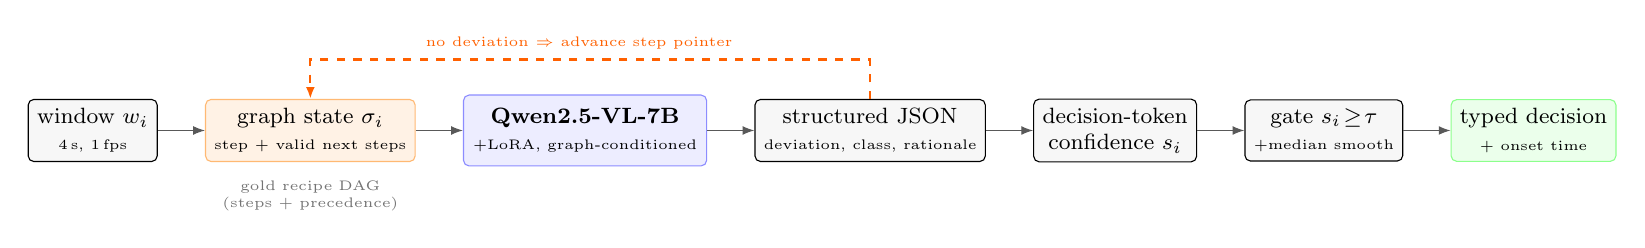
\begin{tikzpicture}[
  font=\footnotesize,
  box/.style   = {draw, rounded corners=2pt, align=center, inner sep=3.2pt,
                  minimum height=7.5mm, fill=black!3},
  vlm/.style   = {draw, rounded corners=2pt, align=center, inner sep=3.5pt,
                  minimum height=9mm, fill=blue!7, draw=blue!45},
  graph/.style = {draw, rounded corners=2pt, align=center, inner sep=3.2pt,
                  minimum height=7.5mm, fill=orange!10, draw=orange!55},
  outbox/.style   = {draw, rounded corners=2pt, align=center, inner sep=3.2pt,
                  minimum height=7.5mm, fill=green!8, draw=green!45},
  ar/.style    = {-{Latex[length=1.5mm]}, draw=black!65},
  fb/.style    = {-{Latex[length=1.5mm]}, draw=orange!75!red, thick, dashed},
]

% ---- perception path
\node[box]                        (win)  {window $w_i$\\{\tiny 4\,s, 1\,fps}};
\node[graph, right=6mm of win]    (state){graph state $\sigma_i$\\{\tiny step +
                                          valid next steps}};
\node[vlm,  right=6mm of state]   (vlm)  {\textbf{Qwen2.5-VL-7B}\\{\tiny +LoRA,
                                          graph-conditioned}};
\node[box,  right=6mm of vlm]     (json) {structured JSON\\{\tiny deviation,
                                          class, rationale}};
\node[box,  right=6mm of json]    (conf) {decision-token\\confidence $s_i$};
\node[box,  right=6mm of conf]    (gate) {gate $s_i\!\ge\!\tau$\\{\tiny +median
                                          smooth}};
\node[outbox, right=6mm of gate]    (dec)  {typed decision\\{\tiny + onset time}};

\foreach \a/\b in {win/state, state/vlm, vlm/json, json/conf, conf/gate, gate/dec}
  \draw[ar] (\a) -- (\b);

% ---- the load-bearing feedback edge
\draw[fb] (json.north) -- ++(0,5mm) -| (state.north)
  node[pos=0.26, above, text=orange!75!red, font=\tiny]
  {no deviation $\Rightarrow$ advance step pointer};

\node[below=1.2mm of state, text width=26mm, align=center, font=\tiny,
      text=black!55] {gold recipe DAG\\(steps + precedence)};

\end{tikzpicture}
}
\caption{\ourmodel{}. Each causal window is judged against the recipe's task
graph at the position the system currently expects. The dashed edge is the
mechanism the method turns on: the graph is \emph{walked} as a state machine
whose transitions are the model's own no-deviation judgements, so a persistent
deviation holds position rather than marching the plan forward without the
person. The confidence that gates the decision is read from the model's
generation logits, not from the confidence field it writes
(Section~\ref{sec:confidence}).}
\label{fig:pipeline}
\end{figure*}

\subsection{Graph representation and graph state}

Each recipe's gold DAG is converted into a typed graph of step nodes with
precedence edges; the dataset's \textsc{start} and \textsc{end} sentinels are
retained as non-executable nodes so every edge endpoint remains valid, and
dangling endpoints are rejected at load time. The 24 recipe graphs range from 9
to 27 steps (mean 16.6).

The state carried across windows is a single pointer $\sigma_i$ into $S$. It
begins at the first step and advances by one whenever the model reports
\emph{no} deviation at $w_i$, clamped at the last step. A persistent deviation
therefore holds the pointer in place: the system waits for the person to come
back to the plan rather than marching on without them. This is the only piece of
inter-window state the method carries besides a three-window judgement history.

\subsection{Graph-conditioned prompting}

At each window the model receives the sampled frames together with a fixed
instruction template filled with: the task name; the current expected step
$\sigma_i$ and its description; the set of valid next steps read off the outgoing
precedence edges; the objects, states, and permitted variations associated with
the step; and a three-window summary of its own recent judgements rendered as
(observed action, deviation flag, predicted class). The template states all
class definitions explicitly, including one-line glosses for the distinctions
most easily confused, and instructs the model to answer with JSON only.

\paragraph{What the conditioning actually contains.} We state plainly what a
reader would otherwise have to discover: although our representation supports
objects, states, and permitted variations, the gold graphs shipped with the
benchmark populate \emph{only} steps and precedence edges. For all 24 recipes the
object, state, and variation fields are empty. Graph conditioning as evaluated in
this paper therefore means \emph{step description, valid next steps, and step
position}, and nothing more. That the effect reported in
Section~\ref{sec:results} is obtained from this much alone is, if anything, the
more interesting reading; but it bounds the claim, and it is why we treat richer
graph content as future work rather than as an established ingredient.

\subsection{Structured output and defensive parsing}

The requested answer has nine fields: observed action, observed objects, matched
step, deviation flag, mistake class, confidence, an uncertainty reason drawn from
a closed vocabulary, a one-to-two sentence rationale, and a brief
expected-versus-observed delta. The JSON object is extracted from the generated
text; the mistake class is validated against $\mathcal{C}$ and the uncertainty
reason against its vocabulary, with out-of-vocabulary values coerced to the safe
default and confidence clamped to $[0,1]$. A total parse failure falls back to a
no-deviation prediction, and the raw text is retained. No parse failures occurred
in any reported run.

\paragraph{Only two fields carry information after fine-tuning.} The schema is
richer than what the fine-tuned model actually uses, and we state this plainly
because the output format invites the opposite assumption. Our supervision
targets are constructed from the window labels alone: the free-text fields are
filled with fixed placeholder strings and the confidence with a constant. The
model reproduces those constants exactly. On a probe of 76 consecutive test
windows the rationale, observed action, observed objects, expected-versus-observed
delta and uncertainty reason each took a \emph{single} value, and the verbalised
confidence was constant at 0.9, while the decision-token probability
(Section~\ref{sec:confidence}) ranged 0.020--0.945 over the same windows.
\textbf{The fine-tuned system is therefore a typed detector, not an explainer};
its informative outputs are the deviation flag, the mistake class, and the
decision-token score. Supervising the free-text fields is left to future work;
the benchmark ships free-text error descriptions that could serve as targets, and we make no claim about explanation quality anywhere in this paper.

\subsection{Decision-token confidence}
\label{sec:confidence}

The model's verbalised confidence field is not a usable signal. Prompted
zero-shot it takes only two distinct values and is statistically indistinguishable
between true and false positives (0.859 vs.\ 0.863). After fine-tuning it is
strictly worse: our supervision targets carry a constant confidence, and the
model reproduces that constant on every window. A constant score makes any
threshold rule inert by construction.

We therefore read the score from the generation logits. Generation is run with
per-step scores retained; the emitted token sequence is walked to the
\texttt{deviation} field and the first subsequent boolean token located. Its
softmax probability is taken as $s_i$, used directly when the model emitted
\emph{true} and complemented when it emitted \emph{false}. If the boolean cannot
be located the fallback is the geometric mean of the emitted tokens'
probabilities, which still varies per window. Figure~\ref{fig:scores} shows
what the two sources look like side by side on the test split.

\begin{figure}[t]
\centering
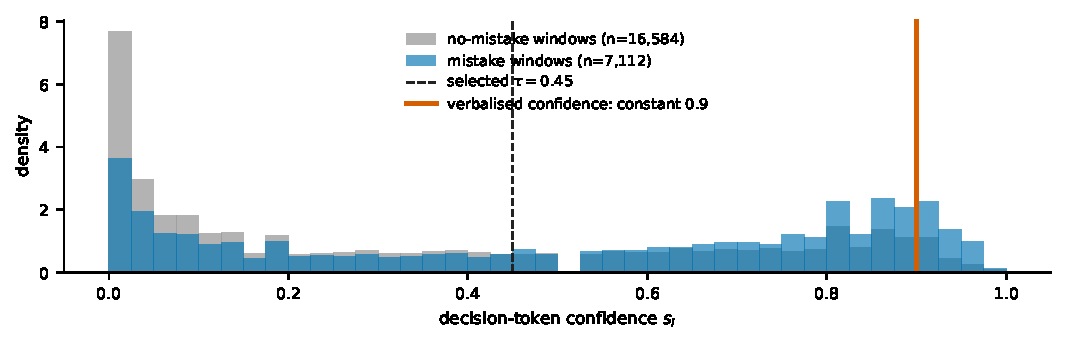
\includegraphics[width=\linewidth]{figures/scores.pdf}
\caption{Where the decision signal comes from. Distribution of the decision-token
confidence $s_i$ on all \resWindows{} test windows, split by ground truth. The two
classes separate (AUC \resAUC{}), with non-mistake windows massed near zero and
mistake windows near 0.8--0.95. The verbalised confidence field, by contrast, is
a single constant on every window (orange), so it supports no ranking at all.}
\label{fig:scores}
\end{figure}
This is a per-window signal with the correct polarity, and
Section~\ref{sec:results} shows it is an informative \emph{ranker}
(AUC \resAUC{}). We are careful not to claim more: it is not calibrated, and we
report calibration error alongside every result so that this is visible rather
than buried.

\subsection{Completion-only LoRA fine-tuning}

We adapt Qwen2.5-VL-7B-Instruct \citep{bai2025qwen25vl} with LoRA
\citep{hu2022lora} of rank 32, scaling 64, dropout 0.05, applied to both attention
(query, key, value, output) and MLP (gate, up, down) projections: 95M
trainable parameters, 1.13\% of the model. The objective is ordinary causal
language-modelling cross-entropy computed \emph{only over the answer tokens},
with prompt and image tokens masked out.

The masking is not a detail. Computing the loss over the full input, roughly
1850 prompt and image tokens against about 71 answer tokens, drowns the
training signal, and in our runs left the loss plateaued near 6.1 without
learning. With completion-only masking the loss falls immediately and converges
to $\approx 0.017$.

One consequence of this design is worth stating for a likely reviewer question:
the mistake taxonomy is never compiled into a classifier head. It lives in the
prompt and in the targets, so the class set can be changed without touching the
architecture.

\subsection{Decision layer}
\label{sec:decision}

Per-window scores become decisions through a small, fully specified layer: a
window fires when $s_i\ge\tau$; a fired window keeps its score and a rejected one
is zeroed; the resulting stream is median-smoothed with width $k$; and the binary
decision is that the smoothed score is positive. The typed stream is gated in
parallel, so that a rejected window is relabelled \texttt{no\_mistake} regardless
of what the model called it. The typed comparison across configurations is then
genuine rather than an artefact of shared intermediates.

Onset localisation deliberately uses a stricter rule than the binary metric: the
predicted onset is the timestamp of the first run of at least $m$ consecutive
fired windows. A recording whose event never fires scores zero earliness and is
excluded from the onset-error mean, with the detected count reported so that the
denominator is auditable.

\paragraph{The one place the pipeline is not causal, and what it costs.}
Every line of Algorithm~\ref{alg:walk} that touches the model is causal, but the
median filter is centred: at width $k=\gateK{}$ a window's smoothed score reads
the two windows after it, so a binary decision and an onset timestamp are
available \csLook{}\,s later than the window they describe. The per-window
judgements and scores are untouched by this, and so are AUC, ECE and Brier,
which never see the filter. We price the rest rather than argue about it, by
replaying the identical saved predictions through a trailing filter of the same
width, which reads only the present and the past. Binary F1 is \csF{} against
\resF{} (\csDelta{}) and the early-detection score \csEDS{} against \resEDS{}
(\csEdsDelta{}); the graph-free arms move the same way and by the same order
(R5 \csNgF{}, R6 \csNtF{}). Every comparison in this paper therefore survives a
strictly causal decision layer, and the ordering of the conditioning variants is
unchanged. We report the centred filter because it is the one selected on
validation and frozen before any ablation existed, not because it is worth
anything. Appendix~\ref{app:causal} gives every arm under both filters.

$(\tau,k,m,\text{gate})$ are selected on the validation split alone: $\tau$,
$k$ and the gate mode by validation binary F1, $m$ by validation early-detection
score at the chosen operating point. The layer is then frozen and applied to test exactly
once. The selected configuration is $\tau=\gateTau$, $k=\gateK$, $m=\gateMinC$;
Appendix~\ref{app:decision} gives the grid.
Each arm receives its own validation-tuned layer, so no arm is advantaged by
threshold placement.


\begin{algorithm}[t]
\small
\caption{\ourmodel{}, one recording. Lines 5--10 are strictly causal: the
prompt, the pointer and the history read only $w_{\le i}$.
\textsc{Advance} is the sole point at which graph state changes, and it is the
only line that differs between the main arm and the corrected-pointer arm
(R11, Section~\ref{sec:graphablation}).}
\label{alg:walk}
\begin{algorithmic}[1]
\Require recording $V$ of task $T$; graph $G_T=(S,E)$; model $f_\theta$;
  decision layer $(\tau,k,m,\textit{gate})$ frozen on validation
\State $\sigma \gets s_1$ \Comment{expected-step pointer}
\State $H \gets \langle\,\rangle$; \; $g \gets \langle\,\rangle$
  \Comment{judgement history; gated scores}
\For{each window $w_i$ of $V$ in temporal order}
  \State $P_i \gets \textsc{Prompt}\big(T,\ \sigma,\ \textsc{Next}(\sigma,E),\ \textsc{Last3}(H)\big)$
  \State $(\hat y_i,\hat c_i) \gets \textsc{ParseJson}\big(f_\theta(w_i,P_i)\big)$
  \State $s_i \gets \Pr\nolimits_\theta[\texttt{deviation}{=}\textsc{true}]$
    \Comment{from the logits, \S\ref{sec:confidence}}
  \State $H \gets H \cup \{(\hat y_i,\hat c_i)\}$
  \State $\sigma \gets \textsc{Advance}(\sigma,\hat y_i)$
    \Comment{deviation holds position}
  \State $\textit{fire}_i \gets [\,s_i \ge \tau\,]$
    \Comment{$[\hat y_i \wedge s_i\ge\tau]$ under \textit{gate}${=}$\textsc{and}}
  \State $g_i \gets s_i \cdot \textit{fire}_i$; \;
         $\tilde c_i \gets \hat c_i$ if $\textit{fire}_i$ else \texttt{no\_mistake}
\EndFor
\State $\bar g \gets \textsc{MedianSmooth}(g,k)$;\quad
       $\hat b_i \gets [\,\bar g_i > 0\,]$
\State $t_{\text{onset}} \gets$ start of the first run of $m$ consecutive fired windows
\State \Return binary stream $\hat b$, typed stream $\tilde c$, onset $t_{\text{onset}}$
\end{algorithmic}
\end{algorithm}

\paragraph{The two step rules.} \textsc{Advance} is instantiated twice in this
paper and nowhere else does the graph arm differ. The rule used for the main
results advances one step at every non-deviant window,
$\sigma \gets \textsc{next}(\sigma)$ if $\neg\hat y_i$, clamped at the last
step. The corrected rule of Section~\ref{sec:graphablation} additionally
rate-limits that advance, requiring a step to be held for
$\lceil \bar d_T/\text{stride}\rceil$ non-deviant windows before it may be left,
where $\bar d_T$ is the mean step duration for task $T$ estimated on the
training split. A deviation holds position under both rules without discarding
progress already made at the current step: with precision \resP{}, isolated
false deviations are common, and resetting would stall the pointer permanently.

% =====================================================================
\section{Experimental Setup}
\label{sec:setup}

\subsection{Benchmark}
CaptainCook4D \citep{peddi2024captaincook4d} contains 384 egocentric recordings
of 24 cooking recipes, about 94.5 hours, with 5700 step segments of which 1964
carry at least one error (2574 error instances), and gold task graphs per recipe.
We use the official split of 213 train / 62 validation / 109 test recordings.
Evaluation covers 14{,}129 validation and \resWindows{} test windows, with zero
recordings dropped and zero graphs missing.

\subsection{Taxonomy and its structural limit}
We adopt the benchmark's native error taxonomy minus the \texttt{Other} catch-all
(8 instances), giving eight classes: \texttt{no\_mistake}, \texttt{order\_error},
\texttt{technique\_error}, \texttt{preparation\_error},
\texttt{measurement\_error}, \texttt{missing\_step}, \texttt{timing\_error},
\texttt{temperature\_error}. Steps carrying several error tags are reduced by a
documented priority in which structural errors outrank execution errors.

One limitation is structural rather than empirical and must be read alongside
every typed result: \texttt{missing\_step} errors are exactly the
non-localisable annotations. A step that never happened produces no video window,
so a windowed detector cannot emit the class: its test support is 2 windows
and its F1 is 0.000 in every row. In practice the method covers 7 of 8 classes,
and we report macro-F1 both with and without it. Sixty-nine non-localisable
segments in the test split are unrecallable by any windowed metric for the same
reason. One further exclusion is small but worth stating: a single step carrying
only the \texttt{Other} tag is dropped from the typed metrics, since that
catch-all is outside our label set. No recording is excluded, and the binary
metrics use every window. Appendix~\ref{app:coverage} gives the per-class support
and the full coverage accounting.

\subsection{Windowing and protocol}
Windows are 4 seconds long, sampled at 1 frame per second, with a 4-second
stride, so windows are contiguous and non-overlapping. A window's ground truth is the
annotation whose span contains the window's midpoint. Windows are emitted while a
full window fits inside the recording, so a trailing remainder shorter than one
stride is left unsampled.

Every result in this paper uses the \textbf{online causal} protocol, with the
single qualification stated and priced in Section~\ref{sec:decision}: the model
never sees the future, and the decision layer's smoothing filter reads
\csLook{}\,s of it, worth \csDelta{} F1. We do not report
an offline (full-video) variant. Earlier versions of this work reported one, and
we drop it deliberately rather than silently: in that implementation the expected
step index was tied to the window index, so it saturated at the final step for
any recording longer than its graph, which is most of them. The offline
condition therefore measured weaker graph conditioning rather than the benefit of
non-causal access, and comparing it against the online rows would have been
misleading. Online is also the setting the task is motivated by: a detector that
needs the rest of the video cannot warn anyone.

\subsection{Metrics}
Binary F1 on the mistake-vs-not decision; macro-F1 and per-class F1 reported with
support, both including and excluding \texttt{missing\_step}; AUC-ROC over the
raw ungated scores, which is threshold-free and therefore comparable across
rows; precision and recall; expected calibration error and Brier score over the
raw per-window scores; and an early-detection score (EDS) with the mean absolute
onset error in seconds. Per-class F1 scores a never-predicted class as $0.0$
rather than dropping it from the average.

\paragraph{Uncertainty.} Every headline metric carries a 95\% percentile
bootstrap interval over 1000 resamples with recordings as the resampling unit
(seed 0), since windows within a recording are strongly correlated. We report a
paired bootstrap over the same resamples for the difference between arms, and a
McNemar test over window decisions as a secondary check.

\subsection{Baseline}
We reproduce MistSense \citep{patsch2025mistsense} end to end and retrain its
Stage-1 detector on CaptainCook4D so that a comparison exists on the same data.
Two deviations are stated for the record: we substitute an ungated LLM
(OPT-2.7b) and CLIP-ViT-L/14 for the paper's gated components; both affect only
the captioning stages, not the detector we compare against. The reproduced
detector scores 0.495 binary F1 on the benchmark under its own native per-frame
protocol with a threshold swept on the test set. That threshold selection is an
oracle and the protocol is not ours, so we do not treat that number as a
comparison. We report a protocol-matched row instead: the baseline's per-frame probabilities are
max-pooled onto our identical \resWindows{} windows, so a window counts as a
mistake if any moment inside it does, and its decision layer is tuned on
validation and frozen, exactly as ours is (selected $\tau=\baseTau$). Coverage is
complete: all \resClips{} test recordings, no missing probability dumps. This is
the only baseline row we treat as comparable, and
Section~\ref{sec:baseline} reads it.

For completeness we also report the baseline under its own native per-frame
protocol with the threshold selected on validation rather than on test: it
reaches 0.452 F1 at $\tau=0.7$, against 0.456 for the best threshold chosen on
test. On that protocol, then, honest threshold selection costs only 0.005. The
larger oracle effect noted above belongs to the coarse 872-window protocol under
which the 0.495 figure was obtained, not to threshold selection in general.

\subsection{Implementation}
Qwen2.5-VL-7B-Instruct in bfloat16 on a single RTX PRO 6000 (96\,GB), greedy
decoding (temperature 0) with a 512-token generation cap, global seed 42. For
fine-tuned evaluation the LoRA adapter is merged into the base weights, so the
fine-tuned and zero-shot runs differ only in weights and are otherwise the same
execution path. Training uses a class-balanced 10{,}000-window subset of the
training recordings (4951 mistake / 5049 normal) drawn at the same window length,
stride and frame rate as evaluation, learning rate $2\!\times\!10^{-4}$ with
cosine schedule and warmup, gradient accumulation 8, two epochs, about three
hours. The window index is built without decoding pixels and frames are decoded
lazily, which is what makes the dataset's $\sim$90k candidate windows tractable.

% =====================================================================
\section{Results}
\label{sec:results}

\begin{table*}[!t]
\centering\footnotesize
\setlength{\tabcolsep}{3.5pt}
\resizebox{\textwidth}{!}{%
\begin{tabular}{lccccccccc}
\toprule
System & binary F1 & P & R & macro F1 & macro F1$^{-}$ & AUC & ECE & EDS & onset MAE (s)\\
\midrule
Zero-shot Qwen2.5-VL, graph prompt & 0.150 \ci{0.127}{0.172} & 0.264 & 0.105 & 0.108 \ci{0.100}{0.115} & 0.123 & 0.480 \ci{0.447}{0.512} & 0.527 & 0.985 \ci{0.971}{0.996} & 64.4 \\
\ourmodel{} (graph prompt + LoRA) & 0.482 \ci{0.392}{0.558} & 0.407 & 0.589 & 0.185 \ci{0.161}{0.208} & 0.212 & 0.636 \ci{0.563}{0.698} & 0.490 & 0.806 \ci{0.705}{0.892} & 60.4 \\
\midrule \ourmodel{} w/o graph at inference (R5) & 0.467 \ci{0.383}{0.536} & 0.419 & 0.527 & 0.191 \ci{0.166}{0.211} & 0.218 & 0.631 \ci{0.564}{0.688} & 0.473 & 0.697 \ci{0.591}{0.801} & 81.5 \\
\ourmodel{} trained \emph{and} tested graph-free (R6) & 0.460 \ci{0.381}{0.534} & 0.453 & 0.467 & 0.186 \ci{0.165}{0.206} & 0.213 & 0.629 \ci{0.560}{0.692} & 0.451 & 0.673 \ci{0.565}{0.778} & 79.6 \\
\ourmodel{} with corrected step pointer (R11) & 0.458 \ci{0.377}{0.542} & 0.303 & 0.933 & 0.082 \ci{0.061}{0.104} & 0.094 & 0.573 \ci{0.484}{0.658} & 0.310 & 0.834 \ci{0.741}{0.912} & 67.3 \\
\midrule MistSense~\citep{patsch2025mistsense}, protocol-matched & 0.477 \ci{0.396}{0.557} & 0.325 & 0.893 & 0.103 \ci{0.096}{0.108} & 0.118 & 0.585 \ci{0.539}{0.630} & 0.454 & 0.991 \ci{0.985}{0.997} & 60.9 \\
\midrule Fire on every window (trivial) & 0.462 & 0.300 & 1.000 & 0.185 & 0.212 & 0.500 & -- & 1.000 & 65.1 \\
\bottomrule%
\end{tabular}}
\caption{Online causal detection on the \textbf{complete} CaptainCook4D test
split: all \resClips{} recordings, \resWindows{} windows, no subsetting. Each arm
uses its own decision layer selected on validation and applied to test once.
Brackets are 95\% clip-level bootstrap intervals (1000 resamples, seed 0).
macro F1$^{-}$ excludes the structurally unreachable \texttt{missing\_step}
class. AUC is computed on raw ungated scores and is therefore threshold-free.
The trivial row fires on every window; read every F1 against it.
ECE is reported for every row because the decision-token score is informative but
uncalibrated (Section~\ref{sec:confidence}); lower is better, and the baseline is
the best-calibrated row. Binary F1 and the localisation columns use different
firing rules by design (Section~\ref{sec:decision}).}
\label{tab:main}
\end{table*}

\subsection{Graph-conditioned fine-tuning}

Table~\ref{tab:main} gives the headline comparison. \ourmodel{} reaches \resF{}
binary F1 against \resZS{} for the identical model, identical prompt, identical
recordings and windows, prompted zero-shot. The paired clip-level bootstrap puts
the difference at \resDelta{} with a 95\% interval of [\resDeltaLo{},
\resDeltaHi{}], and a McNemar test over the \resWindows{} window decisions gives
$p = \resPmc$. Because both rows come from the same recordings, windows, and
protocol, and each received its own validation-tuned decision layer, this is a
like-for-like comparison.

The ranking quality moves further than the F1: AUC over raw scores goes from
\resAUCzs{}, indistinguishable from chance, to \resAUC{}. This matters for
reading the zero-shot row correctly. Its \resZS{} F1 is not evidence that the
zero-shot model detects anything; it is what a validation-tuned threshold can
extract from a near-chance ranker, and its very high EDS reflects indiscriminate
early firing rather than accurate onset detection. Zero-shot Qwen2.5-VL is, on
this task, effectively a non-detector.

\subsection{Isolating the graph}
\label{sec:graphablation}

The comparison in Section~\ref{sec:results} establishes that graph-conditioned
fine-tuning works. It does not, on its own, establish that the \emph{graph} is
what works, because fine-tuning and graph conditioning move together between the
two rows. A model that improved purely by adapting to the benchmark's visual
domain would produce the same table.

We pre-registered four controls, ran two, added a fifth the first two forced on
us, and cancelled the remaining two. Table~\ref{tab:controls} lists all five
beside the main arm and says which is which; Table~\ref{tab:verdict} gives the reading each was
registered to license and the reading it actually licensed. Every control holds
the decision layer of the main row fixed, at the same $\tau$, smoothing width,
persistence and gate mode, frozen on validation before any of these runs
existed, so the only variable is what the model is told about the procedure.

\begin{table}[t]
\centering\small
\setlength{\tabcolsep}{3.5pt}
\begin{tabular}{@{}llccl@{}}
\toprule
Row & Condition & Content & Position & Status \\
\midrule
R4  & Graph-conditioned (main)     & yes   & walked & run \\
R5  & Graph stripped at inference  & no    & ---    & run \\
R6  & Graph-free train and test    & no    & ---    & run \\
R11 & Rate-limited pointer         & yes   & walked & run \\
\midrule
R7  & Deranged (wrong) graph       & wrong & walked & cancelled \\
R10 & Static dump of all steps     & yes   & no     & cancelled \\
\bottomrule
\end{tabular}
\caption{What each control varies, and which we ran. \emph{Content} is whether
the prompt carries this recipe's steps; \emph{position} is whether it also says
where in those steps the person is expected to be. R5 and R6 differ not in
conditioning but in whether the model was ever \emph{trained} with a graph. R7
and R10 were pre-registered and then cancelled: both decompose a detection
effect, and R5 and R6 had by then shown there was none to decompose
(Table~\ref{tab:verdict}).}
\label{tab:controls}
\end{table}

\paragraph{R5: graph stripped at inference.} The fine-tuned model is evaluated
with the graph block removed from the prompt. This measures how much of the
model's behaviour depends on the graph being present \emph{at the moment of
judgement}, as opposed to having been present during training. It is the
cheapest control and the one that most directly addresses the attribution
question.

\paragraph{R6: graph-free training and evaluation.} A second adapter is
trained from the base model under identical hyperparameters, seed, and data, but
with the graph-free prompt throughout, then evaluated graph-free. R5 and R6
together separate two effects that a single graph-off row would conflate: a drop
in R5 alone could mean the model genuinely uses the graph, or merely that it was
trained on a prompt format it is no longer being given. If R6 recovers what R5
loses, the effect was format mismatch; if R6 does not recover it, the graph
carries information the model cannot obtain otherwise.

\paragraph{R7: deranged graph (cancelled).} Every recording is conditioned on a
\emph{different} recipe's graph, under a fixpoint-free permutation with a fixed
seed, so the prompt has exactly the same structure, length and register as the
main arm while its content is wrong. This separates the value of the plan's
content from the value of having any structured scaffold in the context. A
system that performs as well on wrong graphs as on right ones is not using the
plan; it is using the presence of a plan-shaped block.

\paragraph{R10: static dump (cancelled).} The full step list for the correct recipe is
placed in the prompt, but the model is not told where in that list the person
should currently be. This isolates the walked step pointer
(Section~\ref{sec:method}) from the plan itself, and is the control that would
decide whether \emph{walking} the graph is a mechanism or merely an
implementation choice. It too was registered and not run.

\paragraph{How these rows should be read.} We state the interpretation before
reporting the numbers, so that the reading is not selected after seeing them.
Writing $F(\cdot)$ for binary F1 on the frozen decision layer:

\begin{itemize}\itemsep2pt
\item If $F(\text{R4}) \approx F(\text{R5}) \approx F(\text{R6})$, graph
      conditioning contributes nothing measurable and the honest headline is
      that fine-tuning, not the graph, produces the result. The paper's title
      claim would not survive, and we would report it as such.
\item If $F(\text{R4}) > F(\text{R5})$ but $F(\text{R6}) \approx F(\text{R4})$,
      the drop is prompt-format mismatch rather than lost information: the model
      can do as well without the graph provided it was trained that way.
\item If $F(\text{R4}) > F(\text{R6})$ with a clip-level interval excluding
      zero, graph conditioning carries information that graph-free training
      cannot recover, and the central claim holds.
\item If additionally $F(\text{R4}) > F(\text{R7})$, the plan's \emph{content}
      matters and not merely the presence of structure. If $F(\text{R7}) \approx
      F(\text{R4})$, the effect is a prompt-shape artefact and should be
      described that way however favourable R5 and R6 look.
\item If $F(\text{R4}) > F(\text{R10})$, the walked pointer is doing work beyond
      supplying the plan, and the mechanism described in
      Section~\ref{sec:method} is supported. If not, the walk is an
      implementation detail and we say so.
\end{itemize}

Every comparison uses the paired clip-level bootstrap of
Section~\ref{sec:setup}, with recordings as the resampling unit; we treat a
difference whose 95\% interval contains zero as unresolved rather than as
evidence of equivalence, given the interval widths involved.

\paragraph{Results: R5, graph stripped at inference.}
Removing the graph from the prompt costs \ngDelta{} binary F1 (\resF{} $\to$
\ngF{}), with a paired clip-level interval of [\ngDeltaLo{}, \ngDeltaHi{}] that
\emph{contains zero}. The threshold-free ranking is likewise unchanged (AUC
\resAUC{} $\to$ \ngAUC{}, interval containing zero), and macro-F1 does not drop
at all (\resMacro{} $\to$ \ngMacro{}). By the criteria set out above, we cannot
claim a detection-quality effect from graph conditioning at inference: on
everything the detection literature reports, the graph-conditioned and
graph-stripped models are indistinguishable on this benchmark.

One quantity moves, though most of the movement turns out to be firing rate (below). Early detection falls from
\resEDS{} to \ngEDS{}, a paired difference of \ngEdsDelta{} with interval
[\ngEdsLo{}, \ngEdsHi{}] excluding zero, and mean onset error rises from
\resMAE{}\,s to \ngMAE{}\,s. The two systems detect the \emph{same} number of
events (\resDet{} of \resLoc{} in both cases); the graph-conditioned model
detects them \emph{earlier}. This is a coherent reading of the mechanism: the
expected-step pointer tells the model where in the procedure a deviation should
be looked for, which is information about \emph{when} to fire rather than about
\emph{whether} a window is anomalous.

We flag plainly that this is not the result the framing of this paper
anticipated, and we have not rewritten the framing to fit it. The pre-registered
reading applies: on detection quality, the honest statement is that
graph conditioning at inference contributes nothing measurable, and the
zero-shot-to-fine-tuned gap of \resDelta{} is attributable to fine-tuning. What appears to survive is earliness, which we examine under control next. But it is a different claim from the one the title made.

\begin{figure*}[t]
\centering
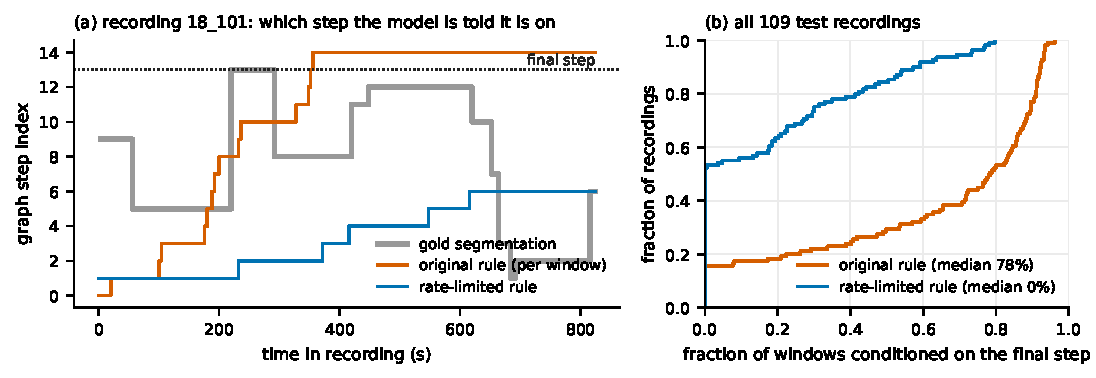
\includegraphics[width=\textwidth]{figures/pointer.pdf}
\caption{The step pointer saturates, and the corrected rule does not.
\textbf{(a)} One test recording of median length. The step the model is told it
is on, over time, under the original per-window rule, the rate-limited rule of
Section~\ref{sec:method}, and the gold segmentation. Both causal rules are driven
by the same deviation flags; only the rule differs. The gold trace also shows
that people do not execute steps in canonical order, so any monotone walk is an
approximation. \textbf{(b)} All 109 test recordings: fraction of windows
conditioned on the final step. Under the original rule the median recording
spends \satMed{}\% of its windows there; under the corrected rule the median is
zero.}
\label{fig:pointer}
\end{figure*}
\paragraph{Why the graph does so little: the pointer saturates.}
The null result on detection has a concrete mechanical cause, which we found by
instrumenting the step pointer rather than by speculating. The pointer advances
by one step for every window the model judges non-deviant, but a recipe step
spans many 4-second windows, so the pointer moves through the graph roughly an
order of magnitude faster than the person does. It therefore reaches the final
step early and clamps there. Across the test split it first reaches the last step
at a median of \satReach{}\% of the way through a recording, and \satPct{}\% of
\emph{all} windows are conditioned on the final step (per-clip median
\satMed{}\%; \satClips{} of 109 recordings spend the majority of their windows
saturated).

For two-thirds of the windows, then, the ``graph context'' is a constant string
naming the last step of the recipe, carrying no information about where the
person actually is. That a graph-conditioned and a graph-stripped model score
identically is exactly what one should expect under that condition. R5 does not
show that procedural structure is useless for this task; it shows that
\emph{this implementation of the pointer stops delivering structure after the
first sixth of a recording}. This is the same saturation failure we
identified in the offline protocol and rejected the protocol for
(Section~\ref{sec:setup}): it is present in the online protocol too, for a
different reason, and we did not notice it until the ablation forced the
question.

\paragraph{And the training signal was worse.} Instrumenting the pointer led us
to check the corresponding assignment during fine-tuning, where we found a
second and larger problem. Training does not use the advancing pointer at all:
it assigns each window the step at its own index, clamped to the last step. A
recipe has 9--27 steps and a recording runs for minutes, so positional variation
exists only in the first $\sim$17 windows, about a minute, of each
recording. Across the training pool, \satTrain{}\% of windows carry the final
step as their graph context (per-recording median \satTrainMed{}\%).

Two consequences follow, and both bear on how the ablation should be read. The
model was fine-tuned on a conditioning signal that was constant for
\satTrain{}\% of its examples, so it had almost no opportunity to learn to use
step position even in principle. And the rule differs between training and
evaluation, so what positional signal did exist at test time was not the signal
the model was trained on. The ablation result is therefore not evidence that a
VLM cannot use procedural structure; it is evidence that this system never
delivered procedural structure to be used.

We report this because it is the most likely reason for the null and because it
was our own defect, found only when the ablation forced us to look. The
correction is not a tuning change: the step assignment must track a person's
progress through the procedure, advancing on evidence that a step has
completed, and it must be the same rule in training and evaluation. That
requires re-training, so it is future work rather than a revision of these
results. Until it is done, this paper's evidence about graph conditioning speaks
to a degenerate delivery of the graph rather than to procedural conditioning in
general, and we would not want the negative result read more broadly than that.

\paragraph{Results: R6, trained and tested without the graph.}
R6 removes the remaining explanation. A second adapter, trained from the base
model on graph-free prompts and evaluated graph-free, reaches \ntF{} binary F1
against \resF{} for the graph-conditioned model. The paired difference is
\ntDelta{} with a 95\% interval of [\ntDeltaLo{}, \ntDeltaHi{}], containing zero;
AUC and macro-F1 likewise show no effect. A model that never saw a procedural
graph, at any point in training or inference, is indistinguishable from
\ourmodel{} on every detection metric we report.

This is the first of the five patterns registered above, and we report it as
such: \textbf{on detection quality, graph conditioning contributes nothing
measurable, and the large gain over zero-shot, \resDelta{} F1, is
attributable to fine-tuning}. The title this paper began with claimed the graph;
that claim does not survive its own ablation, and we have changed the title
rather than qualify it in a footnote.

\begin{figure}[t]
\centering
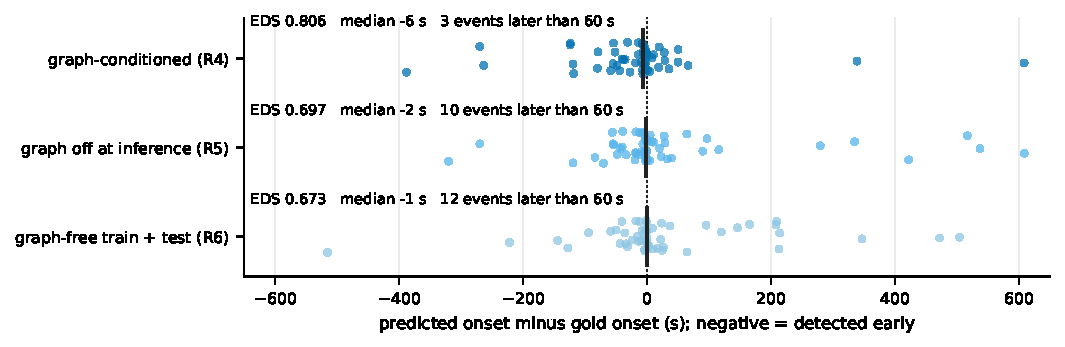
\includegraphics[width=\linewidth]{figures/onset.pdf}
\caption{Onset error before firing rate is controlled for. Predicted minus gold
onset for every detected event, under R4's frozen decision layer, for the three
conditioning variants. The three arms find essentially the same events; the
difference is the tail of late detections, which is what the early-detection
score measures. Read this figure with the matched-event comparison in the text:
restricted to events both arms detect, the graph-conditioned median advantage is
\moMed{}\,s, CI [\moLo{}, \moHi{}].}
\label{fig:onset}
\end{figure}
\paragraph{What appeared to survive, and what is left of it after control.}
One effect was present in both controls: early detection falls from \resEDS{}
to \ngEDS{} without the graph at inference (paired \ngEdsDelta{}, CI
[\ngEdsLo{}, \ngEdsHi{}]) and to \ntEDS{} without it in training (paired
\ntEdsDelta{}, CI [\ntEdsLo{}, \ntEdsHi{}]), both intervals excluding zero, and
Figure~\ref{fig:onset} shows where that difference lives: in the tail of late
detections rather than in which events are found. An
earlier draft of this paper reported that as the graph's contribution. It is
mostly not. The early-detection score rewards firing: a detector that fires on
every window scores \afEDS{}, and the graph-conditioned arm fires more than the
graph-free one (recall \resR{} against \ntR{}). Controlling for detection by
comparing onset error only on events \emph{both} arms found (\moN{} events),
the graph-conditioned model is earlier by a median \moMed{}\,s, with a
bootstrap interval of [\moLo{}, \moHi{}] that touches zero; it is earlier on
\moEarlier{} events and later on \moLater{}. A few seconds, on the edge of
significance, is what remains of the earliness claim once firing rate is held
fixed. We report it as suggestive and no more.

\paragraph{Results: R11, the graph delivered properly.}
The saturation diagnosis above is a claim about our implementation, so we
tested it rather than leaving it as an excuse. We corrected the step assignment
on both sides: training teacher-forces on the benchmark's gold step
segmentation, which cuts the fraction of training windows pinned to the final
step from \satTrain{}\% to 7.5\%, and evaluation uses a causal pointer
rate-limited by per-recipe step durations estimated on the training split,
which cuts evaluation saturation from \satPct{}\% to 20.7\%
(Figure~\ref{fig:pointer}). We retrained the graph arm under otherwise identical
settings and re-ran the full test pass.

It did not help, and the way it failed is the informative part. Binary F1 is
\fxF{} against \resF{} (paired CI containing zero) and AUC falls to \fxAUC{}.
Macro-F1 collapses from \resMacro{} to \fxMacro{} (paired \fxMacroDelta{},
CI [\fxMacroLo{}, \fxMacroHi{}]), because the corrected model has become a
near-constant firer: recall \fxR{} at precision \fxP{}, essentially the trivial
detector of Section~\ref{sec:trivial}. The cause is measurable. The rate-limited
pointer, although it no longer saturates, agrees with the gold step on only
7.7\% of test windows (the original rule: 2.5\%), because people execute steps
out of canonical order and at varying speed (Figure~\ref{fig:pointer}a).
Training had shown the model a correct step on every example; evaluation shows
it a wrong one on 92\% of them. The model fires at 0.958 when the shown step is
right and 0.931 when it is wrong, which is not a mismatch detector but a model
out of its training distribution.

This closes the loop on the diagnosis in a way we did not anticipate. The
original model ignored the graph because training gave it nothing positional to
learn; the corrected model learned to depend on position and was then handed a
position that is almost always wrong. Under a causal protocol with no step
supervision at test time, we do not currently have a way to deliver the graph
accurately enough for a model trained to rely on it. R7 and R10 were not run:
with no detection effect to decompose and the earliness effect reduced to a few
seconds, they no longer bear on any claim this paper makes.
Figure~\ref{fig:ablation} puts the whole comparison in one place: on detection
every variant lies inside every other's interval, and only earliness separates
them. Table~\ref{tab:register} in Appendix~\ref{app:register} lists every row we
produced, including the two guard rows the main table has no space for.

\begin{figure}[t]
\centering
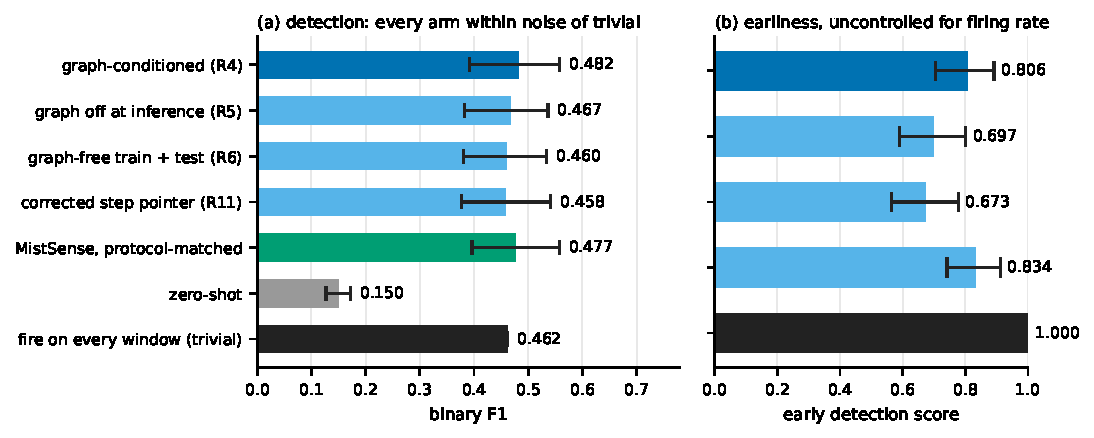
\includegraphics[width=\linewidth]{figures/ablation.pdf}
\caption{Where the effect comes from. \textbf{(a)} On detection, every
conditioning variant lies inside every other's interval, and the whole cluster
sits far above zero-shot: the distance is fine-tuning, not the graph.
\textbf{(b)} On earliness the variants separate, and the paired differences
against R4 exclude zero. Only the three conditioning variants appear in (b):
MistSense (0.991) and zero-shot (0.985) score highest on this metric because
they fire on almost every window, so plotting them here would invite the
misreading the text warns against: early detection is interpretable only
alongside precision. Bars are clip-level bootstrap intervals (1000 resamples,
seed 0).}
\label{fig:ablation}
\end{figure}

\begin{table}[t]
\centering\small
\setlength{\tabcolsep}{3.5pt}
\begin{tabular}{@{}p{0.075\columnwidth}p{0.395\columnwidth}p{0.415\columnwidth}@{}}
\toprule
Test & Registered reading & Verdict on the evidence \\
\midrule
R5 &
$F(\text{R4}){>}F(\text{R5})$ would mean the graph is used at the moment of
judgement &
\textbf{No effect.} \ngDelta{} F1, CI [\ngDeltaLo{}, \ngDeltaHi{}]; AUC and
macro-F1 flat \\[2pt]
R6 &
$F(\text{R4}){>}F(\text{R6})$, interval excluding zero, would carry the
paper's central claim &
\textbf{Claim withdrawn.} \ntDelta{} F1, CI [\ntDeltaLo{}, \ntDeltaHi{}].
Pattern 1 of five obtained; title changed \\[2pt]
EDS &
not registered as primary; examined because it was the one column that moved &
\textbf{Suggestive only.} \ngEdsDelta{} and \ntEdsDelta{} raw, but
\moMed{}\,s (CI [\moLo{}, \moHi{}]) once firing rate is held fixed \\[2pt]
R11 &
if pointer saturation caused the null, repairing it in training and evaluation
should recover an effect &
\textbf{Diagnosis correct, remedy fails.} Saturation \satPct{}\%$\to$20.7\%,
yet F1 \fxF{} and macro-F1 \fxMacroDelta{}: the pointer is right on 7.7\% of
windows \\[2pt]
R7 &
$F(\text{R4}){>}F(\text{R7})$ would separate the plan's content from its shape &
\textbf{Cancelled.} Decomposes an effect R5/R6 showed does not exist \\[2pt]
R10 &
$F(\text{R4}){>}F(\text{R10})$ would show the \emph{walk}, not the plan, is the
mechanism &
\textbf{Cancelled.} Same reason \\[2pt]
R12 &
added after the fact, and it should have been first &
\textbf{Reframes the table.} Firing always scores \afF{}; no learned row is
distinguishable. AUC, \afAucDelta{} CI [\afAucLo{}, \afAucHi{}], is what
separates them \\
\bottomrule
\end{tabular}
\caption{Every test in this paper against the reading it was registered to
license. The R5, R6, R7 and R10 readings are quoted from the list above, which
was written and committed before those runs finished; the R11 reading was
committed before its retrain started. Two of the five registered patterns were
available to us, one obtained, and we report it.}
\label{tab:verdict}
\end{table}

\subsection{The trivial baseline}
\label{sec:trivial}

Table~\ref{tab:main} carries a row we should have computed on day one. On this
split \posRate{}\% of windows are mistakes, so a detector that fires on
\emph{every} window has precision \posRate{}\%, recall 1, and binary F1 \afF{}.
It also scores \afEDS{} on early detection and \afMAE{}\,s onset error, because
it fires at the first window of every recording. No learned system in
Table~\ref{tab:main} is distinguishable from it on binary F1. Ours is
\afDelta{} above it with a paired interval of [\afDeltaLo{}, \afDeltaHi{}]; the
graph-free arm and the corrected-pointer arm are below it; the reproduced
ICCV'25 baseline is \baseF{}. Only the zero-shot model is clearly worse, and it
is worse by under-firing.

This is not a statement that the systems learned nothing. The threshold-free
ranking says otherwise: AUC \resAUC{} against the trivial detector's 0.5, paired
difference \afAucDelta{} with interval [\afAucLo{}, \afAucHi{}], excluding zero
by a wide margin. Fine-tuning produces a genuine ranker. What it does not
produce, at any validation-selected operating point we or the baseline could
find, is an F1 that beats firing indiscriminately. At a 30\% positive rate,
binary F1 on this benchmark is close to a ceiling for any detector that trades
precision for recall, and reporting it without the trivial row invites a
reading the evidence does not support. We recommend that work on this benchmark
report AUC, or precision at fixed recall, alongside F1, and always against this
row.

\subsection{Comparison with prior work}
\label{sec:baseline}

Under the matched protocol MistSense reaches \baseF{} binary F1 against
\ourmodel{}'s \resF{}. The paired clip-level bootstrap puts the difference at
\baseDelta{} with a 95\% interval of [\baseDeltaLo{}, \baseDeltaHi{}]: on
binary detection the two systems are statistically indistinguishable, and we
claim no more than parity. The interval is also wide enough to be
consistent with the baseline being up to 0.06 F1 better. The published
operating point for this baseline (0.495 F1) was obtained by sweeping the
threshold on the test split; when that threshold is instead selected on
validation, as ours is, the apparent margin disappears.

Two caveats bound how much this comparison carries. The baseline is our own
reproduction, and we deliberately did not tune its class weighting
(Section~\ref{sec:setup}); its operating point is far from F1-optimal, and a
better-weighted variant might exceed \resF{}. And it is one recent detector, not
the state of the art: we have not compared against
\citet{lee2026estanet,flaborea2024prego,lee2024egoper} on this benchmark.

\begin{figure}[t]
\centering
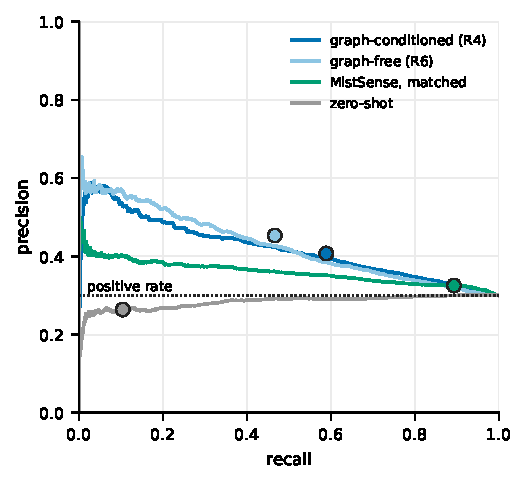
\includegraphics[width=0.78\linewidth]{figures/pr.pdf}
\caption{Precision--recall from the raw ungated scores, with each system's
validation-selected operating point marked. The graph-conditioned and
graph-free curves lie on top of one another, which is the ablation result seen
threshold-free. The baseline reaches its F1 at high recall and low precision;
ours at the opposite end of the same curve.}
\label{fig:pr}
\end{figure}
The two systems arrive at parity by different routes, and
Figure~\ref{fig:pr} shows the routes threshold-free. The baseline achieves its
F1 through recall: it fires on \baseR{} of mistake windows at \baseP{}
precision, and its early-detection score of \baseEDS{} reflects that it is
firing nearly always rather than firing early and correctly. \ourmodel{} is the
more selective of the two (\resP{} precision at \resR{} recall) and ranks
windows better (AUC \resAUC{} vs \baseAUC{}). It also does something the
baseline cannot do at all: it names a mistake type.

The cost of that selectivity should be read alongside it. Firing less often
means catching fewer events: the baseline localises \baseDet{} of \resLoc{}
localisable events and the zero-shot arm \zsDet{}, against \ourmodel{}'s
\resDet{}, at comparable onset error. Which trade-off is preferable depends
entirely on the application, and we do not claim ours is the better operating
point, only that it is a different and more selective one, reached while also
producing a typed label. We record
the macro-F1 column for completeness but do not read it as a comparison. The
baseline is binary by construction, so it cannot score on typing, and the gap
there is definitional rather than empirical.

\subsection{Where the decision signal comes from}

\begin{table}[t]
\centering\small
\setlength{\tabcolsep}{4pt}
\resizebox{\columnwidth}{!}{%
\begin{tabular}{lccccc}
\toprule
Configuration & F1 & P & R & EDS & MAE\\
\midrule
Deviation flag only (no confidence gate) & 0.476 & 0.408 & 0.570 & 0.790 & 61.1 \\
Default gate ($\tau{=}0.5$, AND, $k{=}3$) & 0.471 \ci{0.384}{0.548} & 0.408 & 0.556 & 0.763 & 60.2 \\
Validation-tuned gate (ours) & 0.482 \ci{0.392}{0.558} & 0.407 & 0.589 & 0.806 & 60.4 \\
\bottomrule%
\end{tabular}}
\caption{Decision-layer ablation for \ourmodel{}, all recomputed on CPU from the
same saved predictions. The first row gates on the model's deviation flag alone,
which is what gating on the verbalised confidence reduces to, since that field is
a constant after fine-tuning.}
\label{tab:decision}
\end{table}

Table~\ref{tab:decision} separates the contributions of the decision layer.
Gating on the deviation flag alone, equivalently gating on the verbalised
confidence, which is constant, already recovers most of the performance, and
adding the decision-token confidence with a validation-selected threshold
improves binary F1 modestly. The value of the token-probability score is
therefore not that it rescues the binary decision, but that it exists at all: it
is the only per-window quantity in the system that is continuous, and it is what
makes the threshold-free AUC of \resAUC{}, the score smoothing, and any
downstream operating-point selection possible. With the verbalised field there is
nothing to rank, threshold, or smooth.

\subsection{Typed prediction}

\begin{table}[t]
\centering\small
\begin{tabular}{lrcc}
\toprule
Class & Support & Zero-shot & \ourmodel{}\\
\midrule
\texttt{no\_mistake} & 16,584 & 0.812 & 0.696 \\
\texttt{order} & 4,212 & 0.012 & 0.327 \\
\texttt{technique} & 846 & 0.029 & 0.167 \\
\texttt{preparation} & 621 & 0.009 & 0.060 \\
\texttt{measurement} & 786 & 0.000 & 0.082 \\
\texttt{timing} & 556 & 0.000 & 0.150 \\
\texttt{temperature} & 89 & 0.000 & 0.000 \\
\texttt{missing\_step} & 2 & 0.000 & 0.000 \\
\bottomrule%
\end{tabular}
\caption{Per-class F1 with window support on the test split. Support is severely
imbalanced and two classes are effectively unmeasurable;
\texttt{missing\_step} is structurally unreachable (Section~\ref{sec:setup}).
These are single-run descriptive figures from one training seed
(Section~\ref{sec:limitations}); the ordering of the low-support classes should
not be read as a ranking.}
\label{tab:perclass}
\end{table}

Table~\ref{tab:perclass} reports typed performance, and we read it
conservatively: typing is evidence that the \emph{formulation} reaches
something the binary literature does not, rather than a capability claim. Macro-F1 is \resMacro{} (\resMacroX{} excluding \texttt{missing\_step}).
The system separates mistake from non-mistake well and labels ordering errors
moderately, but it does not reliably name the finer execution types. Two classes cannot be measured meaningfully at all:
\texttt{temperature\_error} has 89 supporting windows and \texttt{missing\_step}
has 2. The honest summary is that \ourmodel{} is a strong binary detector with
partial typing, and the typing is a direction rather than a result.

\subsection{Calibration}

The decision-token score ranks well above chance but is not calibrated, and we
report this rather than leaving it to be inferred. Expected calibration error is
\resECE{} for \ourmodel{} (Brier \resBrier{}), against \baseECE{} for the
baseline: on this axis the baseline is the better-behaved system, and both are
poor in absolute terms. The practical consequence is that the score should be
used for ranking and for threshold selection, which is all our decision layer
does with it, and not read as a probability of error. Calibrating it post hoc
is straightforward and does not change any detection metric, since the standard
mappings are monotone and our operating point is selected on validation either
way; we therefore treat calibration as outside this paper's claims rather than
as a contribution.

\subsection{Onset localisation}

\ourmodel{} detects \resDet{} of the \resLoc{} localisable error events, with an
early-detection score of \resEDS{} and a mean onset error of \resMAE{}\,s. The
onset error is large in absolute terms; recordings in this benchmark run for
several minutes, so \resMAE{}\,s is a coarse but non-trivial localisation.
EDS must be read jointly with precision: a system that fires early and often
scores well on it regardless of accuracy, which is exactly what the zero-shot row
does. Figure~\ref{fig:qualitative} shows two recordings judged over time, both
chosen as failure modes.

\paragraph{What this operating point would mean in use.}
The applications motivating Section~\ref{sec:problem} (assistive guidance,
training, checklists) are worth measuring the result against directly. At
\resP{} precision the system raises roughly three false alarms for every two
correct ones. An assistant that interrupts a cook that often is plausibly worse
than one that stays silent, so we do not claim the system is deployable as an
interrupting assistant. Two readings are more defensible. As a \emph{review}
tool, where a human inspects flagged windows after the fact, this precision is
already useful against \resR{} recall. As an online assistant, the gap to close
is precision at fixed recall, and closing it is future work rather than something
the present numbers support.

\begin{figure*}[t]
\centering
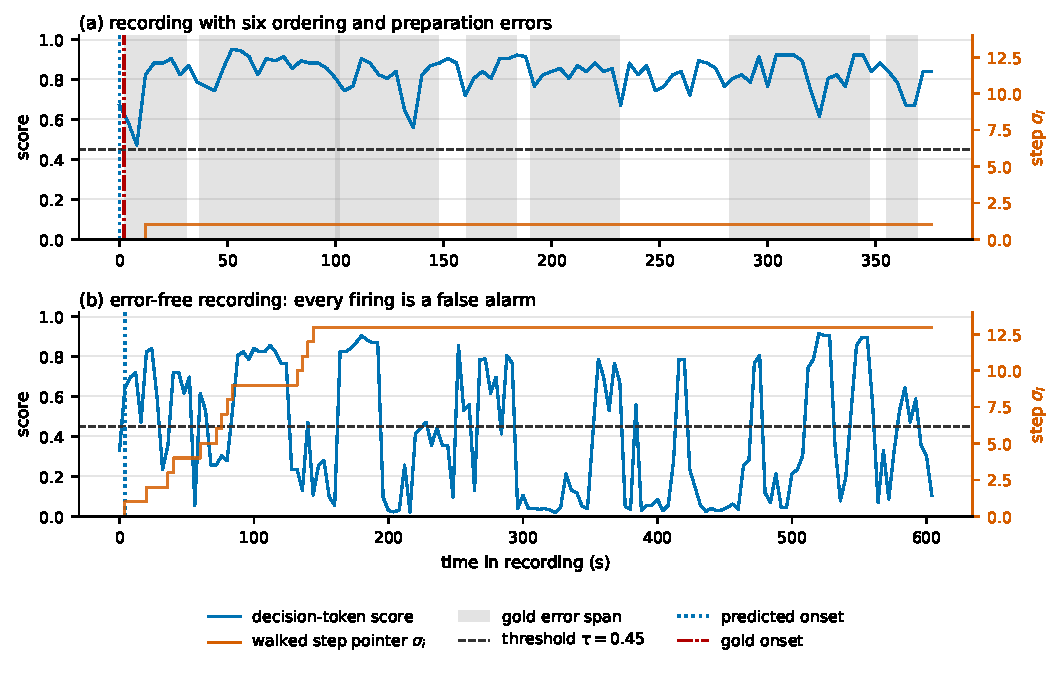
\includegraphics[width=0.92\textwidth]{figures/qualitative.pdf}
\caption{Two recordings judged over time, chosen to show the operating point
honestly rather than favourably. \textbf{(a)} An error-dense recording: the score
sits far above $\tau$ almost throughout, so the system is ``correct'' mainly by
firing continuously, and the pointer consequently stalls near the first step.
\textbf{(b)} An error-free recording, where every one of the 63 firings is a
false alarm, and where the pointer instead runs to the end of the graph within
the first quarter of the recording and clamps, the saturation quantified
above. Both panels are failure modes; with three logged recordings we cannot
also show a clean success, and we prefer to show what the sample contains.}
\label{fig:qualitative}
\end{figure*}

% =====================================================================
\section{Limitations}
\label{sec:limitations}

We state the boundaries of the claim directly.

\textbf{One benchmark, and the claim is scoped to it.} All results are on
CaptainCook4D, in one domain, so every statement here is a statement about
online mistake detection in recorded cooking. We have not shown that any of it
transfers to assembly or laboratory procedures. We considered a second dataset
and did not run one, for a reason worth stating because it constrains the
subfield and not just this paper: the method consumes gold task graphs, and of
the procedural-error benchmarks surveyed in Section~\ref{sec:related}, none
ships them. A transfer study would have to construct the graphs first, which
makes graph quality a confound in the very comparison the study exists to
settle. We would rather make the narrow claim than a wide one resting on graphs
we built ourselves.

\textbf{Graphs are given, not built.} We consume gold task graphs. A deployed
system would need to construct them, and graph quality would then become a
confound; we have not measured the method's sensitivity to graph errors.

\textbf{The conditioning is thinner than the design.} As stated in
Section~\ref{sec:method}, the gold graphs populate only steps and precedence
edges; objects, states, and variations are empty on every window of every run.

\textbf{Operating-point F1 is near trivial.} Firing on every window scores
\afF{}; no learned system in this paper is distinguishable from it on binary F1
(Section~\ref{sec:trivial}). The threshold-free AUC is the evidence of learning.

\textbf{Typing is weak.} Macro-F1 \resMacro{}, with two classes unmeasurable and
one structurally unreachable.

\textbf{The system does not explain itself, though its interface suggests it
could.} The model emits a rationale field, but our supervision fills that field
with a constant, and the fine-tuned model reproduces the constant. We therefore
report no explanation quality and make no interpretability claim. This is a
limitation of how we built the targets rather than of graph conditioning, and
the benchmark's free-text error descriptions are the obvious remedy.

\textbf{The decision layer's filter is not strictly causal.} The model is; the
centred median filter that turns its scores into decisions reads \csLook{}\,s
past each window. We measured the cost of removing it (\csDelta{} F1,
\csEdsDelta{} EDS, Section~\ref{sec:decision}) rather than leaving the reader to
wonder, but a deployment would use the trailing filter and the numbers we report
are the centred ones.

\textbf{Scores are informative but uncalibrated.} The decision-token probability
ranks well above chance but its absolute values should not be read as
probabilities.

\textbf{Single training run.} Every interval we report is an \emph{evaluation}
bootstrap: it covers which recordings were sampled, not which adapter was
trained. The adapter was fine-tuned once, with a single seed, so we cannot
separate the effect of the method from the variance of one training run. We
judge this unlikely to overturn the headline comparison, since the zero-shot to
fine-tuned gap is \resDelta{} with a 95\% interval of [\resDeltaLo{},
\resDeltaHi{}], far wider than plausible seed variance at this scale. But it
does bound the finer-grained claims, and the per-class numbers in particular
should be read as one run rather than an expectation.

\textbf{Baseline comparability.} Our matched row re-tiles the baseline's
per-frame probabilities onto our window grid, which is a fair alignment of
outputs but not a retraining at our frame rate; and our reproduction of it
carries two documented component substitutions. The baseline is also binary by
construction, so the typed columns are not a comparison. Finally, parity is not
superiority: on binary F1 the interval straddles zero.

% =====================================================================
\section{Conclusion}

Giving a vision--language model the plan, and keeping track of
where in the plan the person should be, turns a model that cannot detect
procedural mistakes at all into one that detects them at \resF{} F1 on a full
benchmark test split, names a mistake type, and localises its onset, reaching
parity with a reproduced recent detector under a matched protocol, at a more
selective operating point.

The ablations then took the paper somewhere it did not intend to go, twice. A
model trained and evaluated without any procedural graph matches this one on
every detection metric, so the improvement over zero-shot belongs to
fine-tuning. And once a trivial fire-on-everything detector is placed in the
table, the operating-point F1 that this literature reports turns out to be
within noise of it for every system, ours and the published baseline alike.
What fine-tuning demonstrably produces is a ranker, AUC \resAUC{} against 0.5,
and that is the result we would defend.

We diagnosed the graph's null as a saturating step pointer, corrected it, and
re-ran. The correction made things worse in an instructive way: a model trained
on always-correct steps, then given a causal estimate that is right 7.7\% of
the time, fires on nearly everything. The useful conclusion is therefore not
that procedural structure is useless, but that under a causal protocol without
step supervision we could not deliver it accurately enough for a model to rely
on, and a model that does not rely on it gains nothing from it. Closing that
gap, by supervising step progress directly, is the experiment this paper
motivates and does not run.

% =====================================================================
\section*{Ethics Statement}
This work uses CaptainCook4D \citep{peddi2024captaincook4d}, a publicly released
benchmark of consenting adult participants recorded performing cooking tasks; we
introduce no new human-subjects data and perform no re-identification. The
benchmark is distributed under the Apache License 2.0, which permits the research
use made of it here. Procedural
mistake detection is dual-use: the same capability that supports assistive
guidance and training can support workplace surveillance and productivity
scoring. We note in particular that a detector with this system's precision
(\resP{}) would produce a substantial rate of false accusations if deployed
naively for individual assessment, and we regard per-worker evaluation as an
inappropriate use of this work.

\section*{Use of AI Assistants}
An AI coding assistant was used substantially in this work: in implementing the
evaluation harness, the decision layer, the ablation tooling and the analysis
and plotting scripts, and in drafting and revising this manuscript. Its use was
supervised throughout, and we note two specific practices adopted because of it.
First, every table and every numeric quantity appearing in the prose is
generated programmatically from the saved result artefacts by a single script,
so no reported number is transcribed by hand, by a human or otherwise. Second,
the interpretation of the graph ablation was written and committed to version
control \emph{before} the corresponding runs completed
(Section~\ref{sec:graphablation}), so that the reading of the result could not be
selected after seeing it, a discipline we would recommend regardless of
authorship. Every citation was verified against its published record; one work
asserted in our own planning notes could not be located and was removed rather
than cited. The authors take full responsibility for all content, including the
correctness of every claim, number and reference.

\section*{Reproducibility Statement}
All reported numbers are produced by scripts in the accompanying repository from
saved per-window predictions; the tables in this paper are generated
programmatically from those artefacts rather than transcribed. We report the
random seed, decoding configuration, complete LoRA hyperparameters
(Appendix~\ref{app:hyper}), the exact windowing, and the validation-selected
decision configuration. The prompt templates for all three conditioning variants
are given verbatim in Appendix~\ref{app:prompts}. Code and the saved per-window
predictions, from which every table in this paper is regenerated by a single
script, are available at \coderepo{}; Appendix~\ref{app:repro} gives the two
commands that rebuild every table and figure here.

One reproducibility caveat we state rather than paper over: the dependency
specification pins lower bounds rather than exact versions, so a fresh install
resolves to whatever is current. The exact versions used for the reported runs
are listed in Appendix~\ref{app:hyper}.

\section*{Data and Code Availability}
CaptainCook4D \citep{peddi2024captaincook4d} is third-party and publicly
released by its authors; we redistribute none of it, and the loaders in our
repository read the official release in place. What we release is the
derived material: the saved per-window prediction files for every row in
Table~\ref{tab:main}, the frozen decision parameters, the bootstrap outputs, the
LoRA adapters, and the scripts that turn those into every table and figure here.
The decision layer replays on CPU from the saved predictions and reproduces a
GPU run to floating-point precision, so all re-gating, ablation and bootstrap
numbers are reproducible without a GPU and without re-running inference.

\section*{Conflicts of Interest}
The authors declare no competing financial or non-financial interests. No
funder, and no vendor of any model or tool used here, had any role in the
design, execution, analysis, or reporting of this work.

\section*{Acknowledgments}
\fundingnote{} The disclosure of generative-AI assistance required by ACL policy
is given in full above rather than here, so that it survives anonymisation; it
will be folded into this section at camera-ready, where the policy places it.
The author contribution statement (CRediT) is likewise withheld under anonymous
review.

\bibliographystyle{plainnat}
\bibliography{refs}

\appendix

\section{Complete experiment register}
\label{app:register}

\begin{table*}[!t]
\centering\footnotesize
\setlength{\tabcolsep}{5pt}
\begin{tabular}{@{}llccccccc@{}}
\toprule
& Row & binary F1 & macro F1 & AUC & P & R & EDS & onset MAE (s)\\
\midrule
R1 & Zero-shot, graph prompt, default gate & 0.036 & 0.107 & 0.480 & 0.259 & 0.019 & 0.245 & 236.2 \\
R2 & Zero-shot, graph prompt, val-tuned gate & 0.150 & 0.108 & 0.480 & 0.264 & 0.105 & 0.985 & 64.4 \\
R3 & LoRA + graph, default gate (guard row) & 0.471 & 0.185 & 0.636 & 0.408 & 0.556 & 0.763 & 60.2 \\
R4 & LoRA + graph, val-tuned gate \textbf{(main)} & 0.482 & 0.185 & 0.636 & 0.407 & 0.589 & 0.806 & 60.4 \\
R5 & LoRA + graph, graph stripped at inference & 0.467 & 0.191 & 0.631 & 0.419 & 0.527 & 0.697 & 81.5 \\
R6 & LoRA graph-free, trained and tested & 0.460 & 0.186 & 0.629 & 0.453 & 0.467 & 0.673 & 79.6 \\
R11 & LoRA + graph, corrected step pointer & 0.458 & 0.082 & 0.573 & 0.303 & 0.933 & 0.834 & 67.3 \\
R9 & MistSense, re-tiled, val-tuned gate & 0.477 & 0.103 & 0.585 & 0.325 & 0.893 & 0.991 & 60.9 \\
R12 & Fire on every window (trivial) & 0.462 & 0.185 & 0.500 & 0.300 & 1.000 & 1.000 & 65.1 \\
\midrule
R7 & Deranged (wrong-recipe) graph & \multicolumn{7}{c}{\emph{pre-registered, cancelled unrun (Table~\ref{tab:verdict})}} \\
R10 & Static dump, position removed & \multicolumn{7}{c}{\emph{pre-registered, cancelled unrun}} \\
\bottomrule%
\end{tabular}
\caption{Every row produced under the frozen decision layer, including
the two default-gate guard rows the main table has no room for and the two
controls cancelled unrun. Generated from the same artefact as
Table~\ref{tab:main}, so the two cannot disagree. R1/R3 pair with R2/R4 to show
what validation-tuning the gate is worth on each arm: $+0.114$ F1 zero-shot,
$+0.011$ fine-tuned. R8, the baseline under its own native per-frame protocol
(0.452 F1 at $\tau=0.7$ selected on validation, against 0.456 selected on test),
is deliberately absent: it is not window-matched to any row here and belongs in
prose (Section~\ref{sec:setup}), not in a table with one shared window grid.}
\label{tab:register}
\end{table*}

\section{Prompt templates}
\label{app:prompts}

All three conditioning variants share the same instruction body, the same
eight-class definitions with glosses, and the same JSON output contract; they
differ only in the block describing the procedure. We give that block for each,
since it is the sole experimental variable in Section~\ref{sec:graphablation}.

\paragraph{Graph-conditioned (R4, main arm).}
\begin{quote}\footnotesize\ttfamily
PROCEDURAL GRAPH CONTEXT:\\
Current expected step: \{current\_step\_id\} --- \{current\_step\_desc\}\\
Valid next steps: \{valid\_next\_steps\}\\
Required objects for current step: \{required\_objects\}\\
Expected object states: \{expected\_states\}\\
Valid action variations: \{valid\_variations\}
\end{quote}
As stated in Section~\ref{sec:method}, the last three fields are empty for every
recipe in this benchmark, so the operative content is the current step, its
description, and the valid next steps.

\paragraph{Static dump (R10).}
\begin{quote}\footnotesize\ttfamily
RECIPE STEPS (the full procedure, in order; the person's current position in it
is NOT given):\\
\{all\_steps\}
\end{quote}

\paragraph{Graph-free (R5, R6).} The block is omitted entirely; the model
receives the task name, the frames, and its own recent-judgement summary.

\paragraph{Common to all variants.} The requested answer is a nine-field JSON
object; after fine-tuning only \texttt{deviation} and \texttt{mistake\_class}
carry information (Section~\ref{sec:method}). The recent-history summary renders
the last three windows as (observed action, deviation flag, predicted class).

\section{Hyperparameters and environment}
\label{app:hyper}

\begin{center}
\footnotesize
% Fixed-width value column: with a plain 'l' the long values overran the column
% and bled across the gutter into the neighbouring text.
\begin{tabular}{@{}l@{\hspace{5pt}}p{0.46\columnwidth}@{}}
\toprule
Setting & Value \\
\midrule
Base model & Qwen2.5-VL-7B-Instruct \\
Precision & bfloat16, no quantisation \\
Parameters & 8.29\,B (15.45\,GiB of weights) \\
LoRA rank / scaling / dropout & 32 / 64 / 0.05 \\
LoRA targets & q,k,v,o + gate,up,down \\
Trainable parameters & 95\,M (1.13\%) \\
Objective & completion-only LM cross-entropy \\
Learning rate / schedule & $2\times10^{-4}$ / cosine, 5\% warmup \\
Batch size / grad.\ accumulation & 1 / 8 \\
Epochs & 2 \\
Training windows & 10{,}000 (4951 mistake / 5049 normal) \\
Final training loss & $\approx 0.017$ \\
Adapter size & 364\,MB \\
\midrule
Window length / stride / fps & 4\,s / 4\,s / 1 \\
Decoding & greedy, max 512 new tokens \\
Global seed & 42 \\
Decision layer (val-selected) & $\tau=\gateTau$, $k=\gateK$, $m=\gateMinC$ \\
\midrule
GPU & 1$\times$ RTX PRO 6000, 96\,GiB \\
Inference peak VRAM & 17.5\,GiB allocated, 18.2\,GiB reserved \\
Inference peak host RSS & 16.4\,GiB \\
Training peak VRAM & 55.9\,GiB allocated, 67.5\,GiB reserved \\
Training wall clock & $\approx$3\,h uncontended; $\approx$7\,h shared \\
Full-split inference & 7--24\,h (contention-dependent) \\
\midrule
Python & 3.13.12 \\
torch / CUDA & 2.11.0+cu130 / 13.0 \\
transformers / peft & 5.8.0 / 0.19.1 \\
accelerate & 1.13.0 \\
\bottomrule
\end{tabular}
\captionof{table}{Complete configuration for the reported runs. The
peak-memory figures are instrumented measurements reported by the training and
inference entry points at exit, not estimates.}
\end{center}

\section{Per-class support and coverage}
\label{app:coverage}

Test-split window support by class: \texttt{no\_mistake} 16{,}584;
\texttt{order\_error} 4212; \texttt{technique\_error} 846;
\texttt{measurement\_error} 786; \texttt{preparation\_error} 621;
\texttt{timing\_error} 556; \texttt{temperature\_error} 89;
\texttt{missing\_step} 2. Coverage accounting for every reported run: 109 of 109
recordings evaluated, 23{,}696 windows, zero graphs missing, zero frames
dropped, 61 localisable events, 69 non-localisable segments, and one
\texttt{Other}-only step excluded from typed metrics.

\section{Strictly causal decision layer}
\label{app:causal}

The reported decision layer smooths with a centred median filter, which reads
\csLook{}\,s past each window (Section~\ref{sec:decision}). Replaying the
identical saved predictions through a trailing filter of the same width gives a
strictly causal system: binary F1 \resF{}~$\to$~\csF{}, \ngF{}~$\to$~\csNgF{}
(R5) and \ntF{}~$\to$~\csNtF{} (R6); early detection \resEDS{}~$\to$~\csEDS{},
\ngEDS{}~$\to$~\csNgEDS{} and \ntEDS{}~$\to$~\csNtEDS{}. The main arm is
marginally \emph{better} strictly causal and the graph-free arms marginally
worse, so the ordering of the conditioning variants and every interval-based
conclusion in Section~\ref{sec:graphablation} is unchanged. Reproduce with
\texttt{scripts/cc4d\_causal\_smoothing.py}.

\section{Decision-layer selection}
\label{app:decision}

The layer is selected by grid search on the 62-recording validation split over
$\tau \in [0.30, 0.90]$ in steps of 0.025, smoothing width $k \in \{1,3,5\}$,
gate mode $\in$ \{AND, confidence-only\}, chosen by validation binary F1;
persistence $m \in \{1,2,3\}$ is then chosen by validation early-detection score
at that operating point, since $m$ cannot affect binary F1. The selected
configuration is applied to the test split exactly once. Each arm receives its
own selection, so no arm is advantaged by threshold placement; the graph-ablation
rows deliberately reuse the main arm's frozen layer so that conditioning is the
only variable.

\section{Reproducing every number}
\label{app:repro}

Every table and every numeric quantity in the prose is generated from the saved
per-window predictions by one command:

\begin{quote}\scriptsize\ttfamily\raggedright
python paper/gen\_tables.py\\
cd paper \&\& latexmk -pdf main.tex
\end{quote}

That regenerates the manuscript from artefacts. Regenerating the artefacts
themselves splits into one expensive stage and one cheap one, and the split is
the point: only the first needs a GPU.

\paragraph{GPU, once per arm.} Collecting per-window predictions is the only
step that runs the model. Each pass is 7--24\,h depending on contention and is
restart-safe at one-recording granularity, so an interrupted run is re-issued
verbatim.

\begin{quote}\scriptsize\ttfamily\raggedright
\# R4, the main arm\\
python scripts/cc4d\_collect\_preds.py --split test --stride 4 \textbackslash\\
\hspace*{1em}--lora\_adapter outputs/lora\_cc4d\_8class \textbackslash\\
\hspace*{1em}--save\_preds .../lora\_test\_preds.json\\[3pt]
\# R5: same adapter, graph block stripped\\
\hspace*{1em}--prompt\_variant nograph\\[3pt]
\# R6: adapter retrained graph-free, evaluated graph-free\\
\hspace*{1em}--lora\_adapter .../8class\_nograph \textbackslash\\
\hspace*{1em}--prompt\_variant nograph\\[3pt]
\# R7, had it been run: content wrong, shape identical\\
\hspace*{1em}--graph\_permute\_seed 0
\end{quote}

\paragraph{CPU, everything else.} The decision layer replays from a saved
predictions file and reproduces a GPU run to floating-point precision, so every
re-gate, interval, ablation row and figure below is regenerable in minutes on a
laptop, with no GPU and no model download.

\begin{quote}\scriptsize\ttfamily\raggedright
\# select the layer on val, freeze it, apply once to test\\
python scripts/cc4d\_decision\_sweep.py --arm lora \textbackslash\\
\hspace*{1em}--val\_preds ... --test\_preds ...\\[3pt]
\# apply a frozen layer to any other arm\\
python scripts/cc4d\_decision\_eval.py --preds ... --split test \textbackslash\\
\hspace*{1em}--tau 0.45 --smooth\_k 5 --min\_consecutive 1 \textbackslash\\
\hspace*{1em}--gate\_mode conf\_only --out row\_*.json\\[3pt]
\# clip-level bootstrap; --preds\_b makes it paired\\
python scripts/cc4d\_bootstrap\_compare.py --preds ... \textbackslash\\
\hspace*{1em}--params ... --preds\_b ... --label ...\\[3pt]
\# Table 6, from the manifest of rows\\
python scripts/cc4d\_build\_ablation.py --manifest ...\\[3pt]
\# Figure 3, and the saturation percentages in \S6.2\\
python scripts/cc4d\_pointer\_analysis.py\\[3pt]
\# the matched-event onset comparison of \S6.2\\
python scripts/cc4d\_matched\_onset.py\\[3pt]
\# Appendix E, the strictly causal decision layer\\
python scripts/cc4d\_causal\_smoothing.py --preds R4=... R5=... \textbackslash\\
\hspace*{1em}--params ... --out causal\_smoothing.json\\[3pt]
\# the protocol-matched baseline row (R9)\\
python scripts/cc4d\_mistsense\_retile.py
\end{quote}

\paragraph{What is fixed and what is not.} The seed (42), the decoding
configuration (greedy, temperature 0), the bootstrap seed (0) and the frozen
decision parameters are all pinned, so the CPU stage is deterministic. The GPU
stage is deterministic up to the usual kernel non-determinism in bf16 attention.
The dependency specification pins lower bounds rather than exact versions
(Appendix~\ref{app:hyper} lists the versions actually used), which is the one
place a fresh install can drift from our numbers.

\end{document}
